\documentclass[12pt,fleqn]{report}%type of document, with different options
% fleqn - floats left equations. If you want them centered, remove it.

%different packages
\usepackage{graphicx}
\usepackage{mathtools}
\graphicspath{ {images/} }

\usepackage{url}

\usepackage{braket}

\usepackage{subcaption}

\usepackage[utf8x]{inputenc}



%noi comenzi pentru a redenumi componentele în română
\renewcommand{\chaptername}{Capitolul}
\renewcommand{\contentsname}{Cuprins}
\renewcommand{\appendixname}{Anexa}
\renewcommand{\appendixname}{Anexa}
\renewcommand{\figurename}{Figura}
%\renewcommand\refname{New Title}-pentru articol
\renewcommand\bibname{Bibliografie} %book or report

%numai daca aveti anexa
\usepackage[titletoc]{appendix}

%page style
\setlength{\parindent}{0pt}
\setlength{\topmargin}{-0.2in}
\setlength{\oddsidemargin}{0.5in}
\setlength{\evensidemargin}{0.5in}
\setlength{\textwidth}{15cm}
\setlength{\textheight}{22cm}

\setlength{\parskip}{10pt plus 1pt minus 1pt}

\setlength{\parindent}{1cm}

\usepackage{setspace}
\linespread{1.5}


% Romanian characters shortcuts - redundant for new operation systems - you can select Romanian standard keyboard and \usepackage[utf8x]{inputenc} deja introdus mai sus
\newcommand{\ab}{\v{a}} 
\newcommand{\ac}{\^{a}} 
\newcommand{\ib}{\^{\i}} 
\newcommand{\tb}{\c{t}} 
\newcommand{\st}{\c{s}}
\newcommand{\Ab}{\v{A}} 
\newcommand{\Ai}{\^{A}} 
\newcommand{\Ib}{\^{I}} 
\newcommand{\Tb}{\c{T}}
\newcommand{\St}{\c{S}}

% you can introduce shortcuts for anything else, but without overlaping predefined LaTeX commands
\newcommand{\HRule}{\rule{\linewidth}{0.4mm}}

\begin{document}
	
\begin{titlepage}
	\begin{center}
		
		
		\begin{tabular}{lcr}
			
			
			
\includegraphics[width=2.5cm]{unibuc.jpg} &
			
			\begin{tabular}{c}
				{\large \textsc{Universitatea din București}} \\
				{ \large \text{Facultatea de Fizică}}\\
				\\
				\\
				\\
				\\
				\\
			\end{tabular}
			& 
\includegraphics[width=3.3cm]{fizica}
		\end{tabular}
		
		
		\vspace{2cm}
		
		{\Large Prenume NUME}\\[1.1cm]
		
		\HRule \\[0.3cm]
		
		
		{\Large \textsc {Titlul tezei}}\\
		
		%%	\rule{4cm}{0.5pt}\\[0.4cm]
		
		%%  {\LARGE \textsc{Subtitlul raportului}}\\[0.1cm]
		
		\HRule \\[1.1cm]
		
		\textsc{\large Lucrare de licen\tb\ab}\\[3cm]
		
		% Autor ?i supervizor
		\begin{minipage}{0.45\textwidth}
			\begin{flushleft} \large
				%%    \emph{Autor:}\\[0.1cm]
				%%    Prenume  \textsc{Nume}
			\end{flushleft}
		\end{minipage}
		\begin{minipage}{0.45\textwidth}
			\begin{flushright} \large
				{Conduc\u{a}tor \c{s}tiin\c{t}ific} \\[0.1cm]
				Lect.dr.\ Roxana ZUS \\
				Prof.dr.\ Virgil B\Ab RAN
			\end{flushright}
		\end{minipage}
		
		\vfill
		
		% Partea de jos a paginii
		%% {\large \today}
		
		{\large Bucure\c{s}ti, 2017}
		
	\end{center}
	
\end{titlepage}  
	
	\newpage
	
	\thispagestyle{empty}
%\phantom{Hallo!}
\newpage

\pagenumbering{roman}
\tableofcontents
\cleardoublepage
\pagenumbering{arabic}

%\listoffigures
%\listoftables

	
	\documentclass[12pt, class=report, crop=false]{standalone}
\usepackage{ba_thesis}

\begin{document}

% \addcontentsline{toc}{chapter}{Introduction}
\chapter{Introduction}%
\label{chap:intro}

In this thesis \dots

%\section*{Acknowledgments}
%I would like to thank my advisers, Prof.~dr.~Virgil Băran and Conf.~dr.~Alexandru Nicolin,
%for their help.

\end{document}



	
		
%%%%%%%%%%%%%%%%%%%%%%%%%%%%%%%%%%%%%%%%%%%%%%%%%%%%%%%%%%%%%%%%%%
\chapter{Atomul hidrogenoid - metoda polinomială}
\label{atom}
%%%%%%%%%%%%%%%%%%%%%%%%%%%%%%%%%%%%%%%%%%%%%%%%%%%%%%


\indent

\par Prezentam mai jos principalele etape de calcul si rezultatele pentru miscarea in camp Coulombian: atomul hidrogenoid. Pentru alternative, pot fi urm\ab rite calculele din \cite{Zet09,Sak93}.

Pentru descrierea miscarii in camp central in general, putem considera o microparticula de masa $m_{0}$ care se misca intr-un camp de forte generat de
\begin{equation}
\label{forta}
\overrightarrow{F}=-\nabla_{\overrightarrow{r}}V(r)=-\overrightarrow{e}_{r}\frac{\partial V(r)}{\partial r}
\end{equation}
 Se rezolva problema de functii si valori proprii pentru operatorul asociat energiei (Hamiltonianul), corespunz\ab tor poten\tb ialului din ecua\tb ia (\ref{forta}):
 \begin{equation}
 H \ket{u} = E \ket{u} ,
 \end{equation}
 unde în reprezentarea poziției
 \begin{equation}
 H=-\frac{\hbar^{2}}{2m_{0}}\left(\frac{1}{r^{2}}\frac{\partial}{\partial r}\left(r^{2}\frac{\partial}{\partial r}\right)-\frac{1}{r^{2}}\frac{\overrightarrow{L}^{2}}{\hbar^{2}}\right)+V(r).
 \end{equation}
 Datorita faptului ca $H$, $\overrightarrow{L}^{2}$ si $ L_{z} $ comuta intre ei, adica:
 \begin{equation}
 \begin{split}
		\left[H,\overrightarrow{L}^{2}\right] &=0 \\
		\left[H,\overrightarrow{L}_{z}\right] &=0 \\
		\left[\overrightarrow{L}^{2}, \overrightarrow{L}_{z}\right] &=0 
		\end{split}
 \end{equation}
 $E$, $\overrightarrow{l}^{2}$, $l_{z}$ formeaza un sistem complet de observabile compatibile.

    \begin{figure}[h!]
    	\centering
    	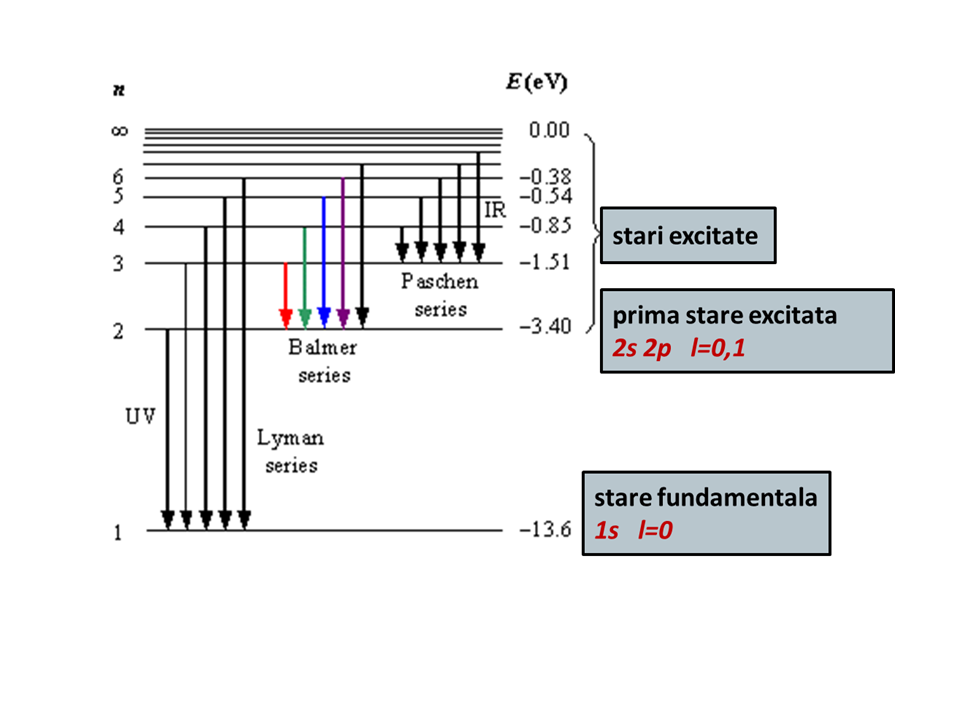
\includegraphics [width=1\textwidth]{poza-nivele-energie}
    	\caption{Nivele de energie si exemple de tranzitii intre acestea (cu spectre in domeniul UV, vizibil si IR).}
    	\label{niveleatom}
    \end{figure}
În figura \ref{niveleatom} .....
			

\chapter{Summary and Outlook
 }
\label{so}
%\chaptermark{}
%%%%%%%%%%%%%%%%%%%%%%%%%

\indent

Scopul acestei lucr\ab ri  a fost studiul/ investigarea ....

Capitolul 2 a fost dedicat...

In ultima parte a lucrarii am studiat ...

Eventual idei pentru teme viitoare
 






















%numai daca aveti anexa


%anexa este optionala, dar pot fi si mai multe anexe, fiercare cu titlul ei, la chapter

\begin{appendices}
	%%%%%%%%%%%%%%%%%%%%
	\chapter{Integrale} 
	\label{anexa1}
	%%%%%%%%%%%%%%%%%%
	
	
	\begin{table}[h]
		\centerline{
			\begin{tabular}{|c|c|c|c|} %cate coloane are
				\hline
				% & &  & \\
				Rule & No. of points/ $[a,b]$ & $h$ & Formula for $I=\displaystyle\int_a^b{f(x)} dx$ \\
				% & Interval $[a,b]$& & $I=\displaystyle\int_a^b{f(x)}$ \\
				\hline
				\hline
				& &  & \\
				Simpson &  $3$ points: $[x_0,x_2]$& $h=\displaystyle\frac{b-a}{2}$ & $I \simeq \displaystyle\frac{h}{3}(f_0 + 4f_1 + f_2) + {\cal O}(h^5) $ \\ 
				\hline				
				& &  & \\ %rand gol
			coloana 1 &  2 & 3 & 4 \\ 
				\hline
			\end{tabular}
		}
		\caption{\label{cfni} Closed formulas for numerical integration.}
	\end{table}
	
	%%%%%%%%%%%%%%%%%%
	\chapter{Alta anexa}
	\label{anexa2}
	%%%%%%%%%%%%%%%%
	
	
	
	
\end{appendices}

\begin{thebibliography}{99}

\bibitem [Jam14]{Jam14} David M. Jameson, {\it Introduction to Fluorescence}, CRC Press, Taylor \& Francisc Group, Boca Raton FL, 2014
\bibitem [Lak06]{Lak06} Joseph R. Lakowicz, {\it Principles of Fluorescence Spectroscopy}, 2006
\bibitem [Han13]{Han13} Dr. Jonas Hannestad, {\it Fluorescence in Bio-inspired Nanotechnology}, 2013
\bibitem [Jam11]{Jam11} David Jameson {\it Principles of Fluorescence Techniques}, first edition, 2011
\bibitem[Mes99]{Mes99} A. Messiah, {\it Quantum Mechanics},  Dover Publications, 1999
\bibitem[Sak93]{Sak93} J.J. Sakurai, {\it Modern Quantum Mechanics }, Addison Wesley; Revised edition, 1993
\bibitem[Zet09]{Zet09} N. Zettili, {\it Quantum Mechanics Concepts and Applications }, second edition, John Wiley \& Sons, 2009
\bibitem [Dan10]{Dan10} Andrei Florin Danet, {\it Analiza instrumentala}, Editura Universitatii din Bucuresti, 2010

{\bf Resurse web:}

\bibitem{1} \url{ http://micro.magnet.fsu.edu/primer/java/jablonski/lightandcolor/ }
\bibitem{2}  \url{ http://hyperphysics.phy-astr.gsu.edu/hbase/quantum/imgqua/qhareig }
\bibitem{3}  \url{ http://hyperphysics.phy-astr.gsu.edu/hbase/quantum/imgqua/qhareig }
\end{thebibliography}
\addcontentsline{toc}{chapter}{Bibliografie}






\let\cleardoublepage\clearpage

\end{document}